\documentclass[hyperref=colorlinks]{beamer}
\mode<presentation>
\usetheme{iclpt}
\setbeamertemplate{navigation symbols}{}
\setbeamertemplate{headline}{
\begin{beamercolorbox}[leftskip=.2cm,rightskip=.2cm,topskip=.2cm,ht=1.1cm,dp=0.1cm,wd=\textwidth]{institute in head/foot}
  
\includegraphics[height=1cm]{icl.pdf}
  \hfill
  
\includegraphics[height=1cm]{../Pics/CMS-Color.pdf}
\end{beamercolorbox}
}
\setbeamertemplate{footline}{
\begin{beamercolorbox}[ht=.55cm,dp=0.4cm,wd=\textwidth,leftskip=.3cm]{author in head/foot}%
  \begin{minipage}[c]{5cm}%
    \usebeamerfont{author in head/foot}
    \insertshortauthor 
    \insertshorttitle
    \end{minipage}\hfill%
  \insertframenumber{} / \pageref{lastframe}
  \hfill
  \begin{minipage}{6cm}
    \hfill
  \end{minipage}
\end{beamercolorbox}%
}

\usepackage{color}
\usepackage{tabularx,colortbl}
\usepackage{graphicx}
\usepackage{pdfpages}
\usepackage{feynmp}
\DeclareGraphicsRule{*}{mps}{*}{}

\title{\vspace{-0.2cm} BDT first look}
%\subtitle{Paper - HIG-13-030, PASs: HIG-13-013, HIG-13-018, HIG-13-028 \vspace{-0.7cm}}
\author[P. Dunne]{\underline{P. Dunne} }%\\ on behalf of the H$\rightarrow$invisible analysis groups} % A.M. Magnan and A. Nikitenko Joao Pela with \\ R. Aggleton, J. Brooke: Bristol \\ C.Asawangtrakuldee, Q.Li: Peking \\ P. Srimanobhas: Chulalongkorn \\ S. Kumar, K. Mazumdar: Mumbai}
\titlegraphic{
  \vspace{-0.7cm}
  %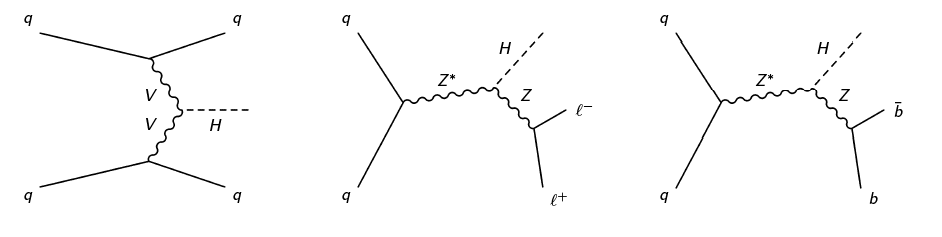
\includegraphics[width=\textwidth]{TalkPics/invcomb021213/feyndiags}
%% \begin{fmfgraph*}(100,70)
%%         \fmfleft{i1,i2}
%%         \fmfright{o1,o2,o3}
%%         \fmf{fermion}{i1,v1,o1}
%%         \fmf{fermion}{i2,v2,o3}
%%         \fmf{phantom,tension=4/5}{v1,v2}
%%         \fmffreeze
%%         \fmf{photon,label=$W,,Z$}{v1,v3}
%%         \fmf{photon,label=$W,,Z$}{v2,v3}
%%         \fmf{dashes}{v3,o2}
%%         \fmflabel{$q$}{i1}
%%         \fmflabel{$q$}{i2}
%%         \fmflabel{$q$}{o1}
%%         \fmflabel{$q$}{o3}
%%         \fmflabel{$H$}{o2}
%%       \end{fmfgraph*}
}
\date{}
\begin{document}
\begin{fmffile}{hig1330approvalfeynmandiags}

%TITLE PAGE
\section{Title}
\begin{frame}
  \titlepage
  
\end{frame}

%OUTLINE

\begin{frame}
  \frametitle{Updates}
  \begin{itemize}
  \item AN rough draft ready for reading: caveats sent in email to the list
  \item Phat noticed an error in the lumi calculation for run B
  \item[-] Jobs rerunning with correct lumi weighting and trigger efficiency average
  \end{itemize}
\end{frame}

\begin{frame}
  \frametitle{BDT Intro}
    \begin{block}{}
      \scriptsize
      \begin{itemize}
      \item Have taken a very quick look at the BDT
      \item Have got data driven weights for backgrounds
      \item Start from signal region of cut based analysis
      \item Caveats:
      \item[-] Z samples not properly accounted for yet: this is being taken care of but samples aren't ready yet
      \item[-] Lumi bug mentioned by Phat yesterday not fixed in these slides - should be small effect
      \item[-] Haven't got expected limit effects
      \end{itemize}
    \end{block}
\end{frame}

\begin{frame}
  \frametitle{List of variables used}
  \begin{block}{}
    \begin{columns}
      \column{.53\textwidth}
    \begin{itemize}
    \item  alljetsmetnomu\_mindphi
    \item dijetmetnomu\_ptfraction
    \item dijetmetnomu\_vectorialSum\_pt
    \item dijetmetnomu\_scalarSum\_pt
    \item n\_jets\_cjv\_30
    \item jet1\_pt
    \item jet2\_pt
    \item dijet\_M
    \item dijet\_deta
    \end{itemize}
      \column{.5\textwidth}
      \begin{itemize}
    \item dijet\_sumeta
    \item dijet\_dphi
    \item metnomuons
    \item metnomu\_significance
    \item sqrt(ht)
    \item ht
    \item jetunclet\_mindphi
    \item metnomuunclet\_dphi
    \end{itemize}
    \end{columns}
  \end{block}
\end{frame}

\begin{frame}
  \frametitle{Correlation Plots}
  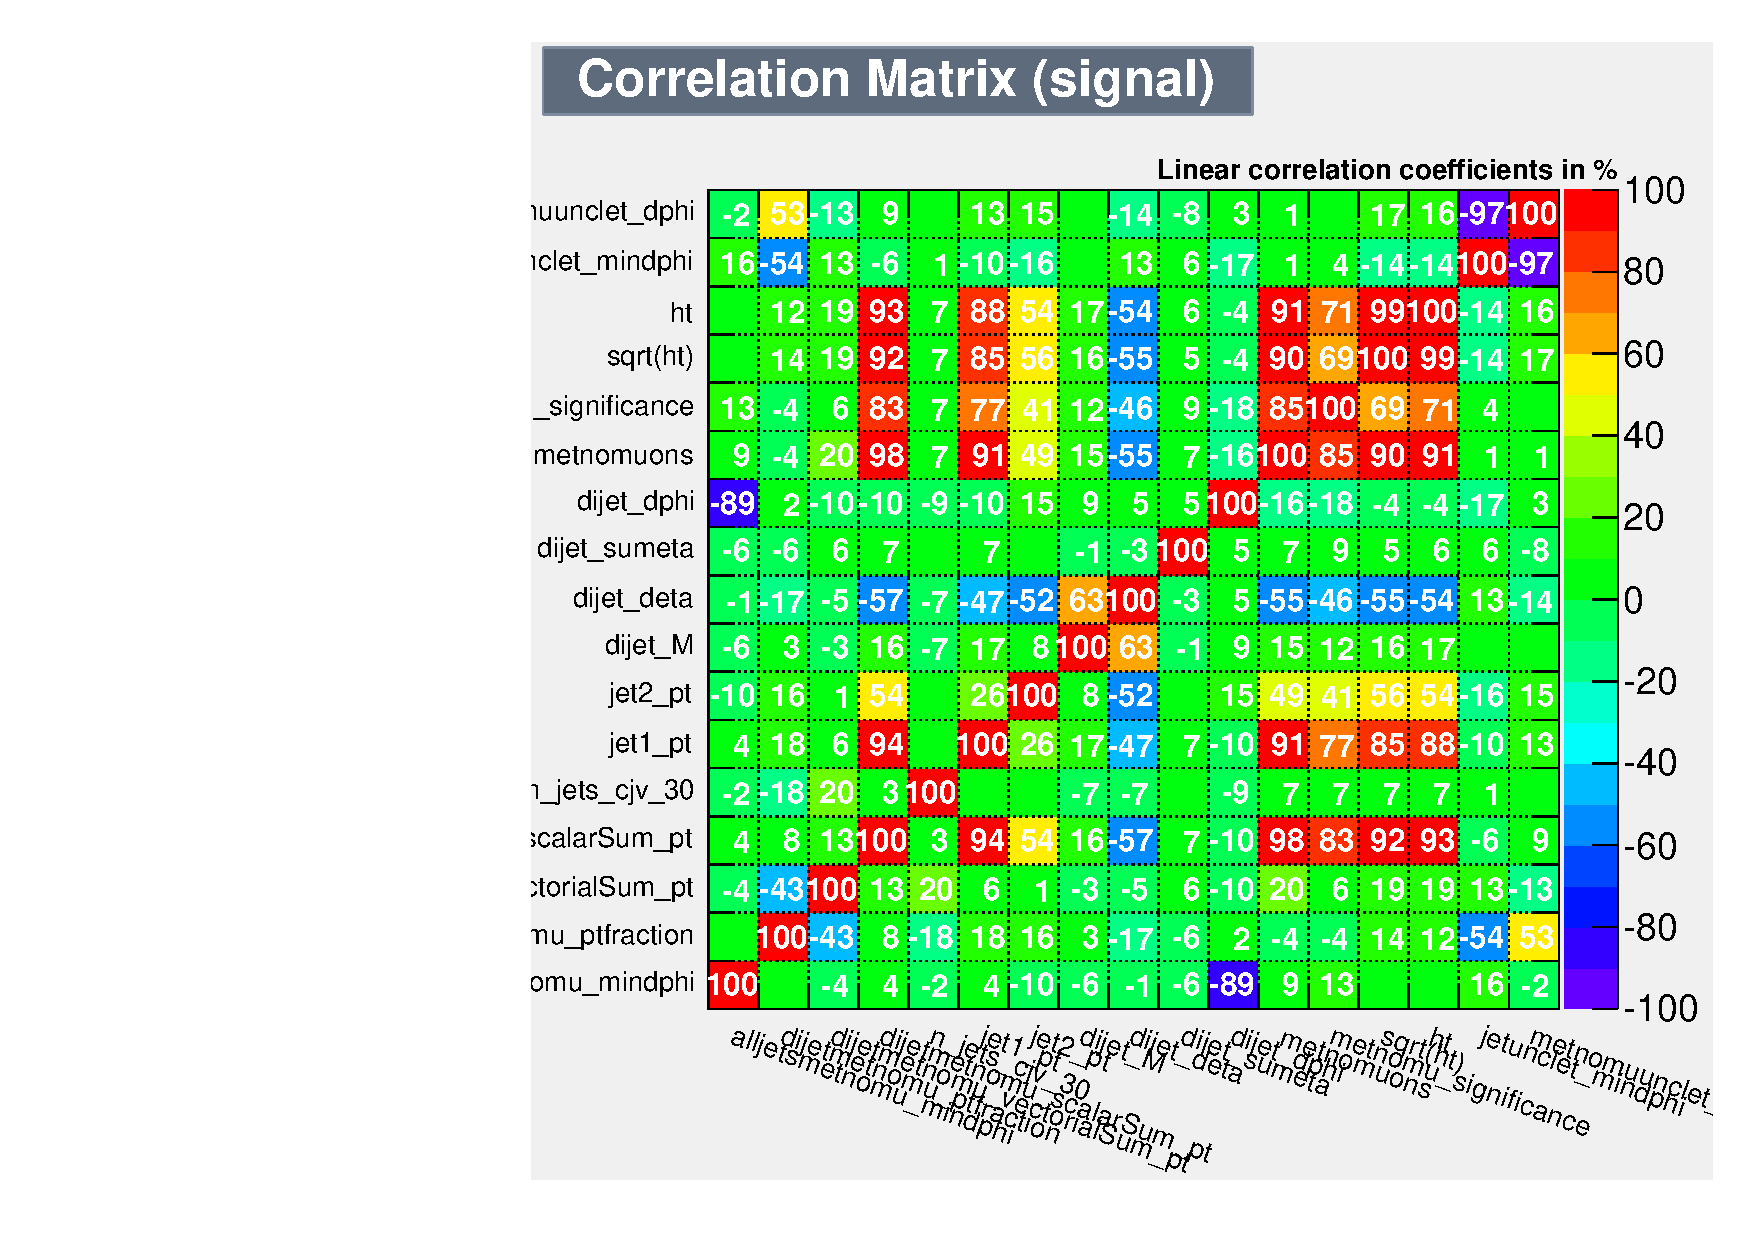
\includegraphics[width=0.5\textwidth]{TalkPics/bdt271014/sigcorr.pdf}
  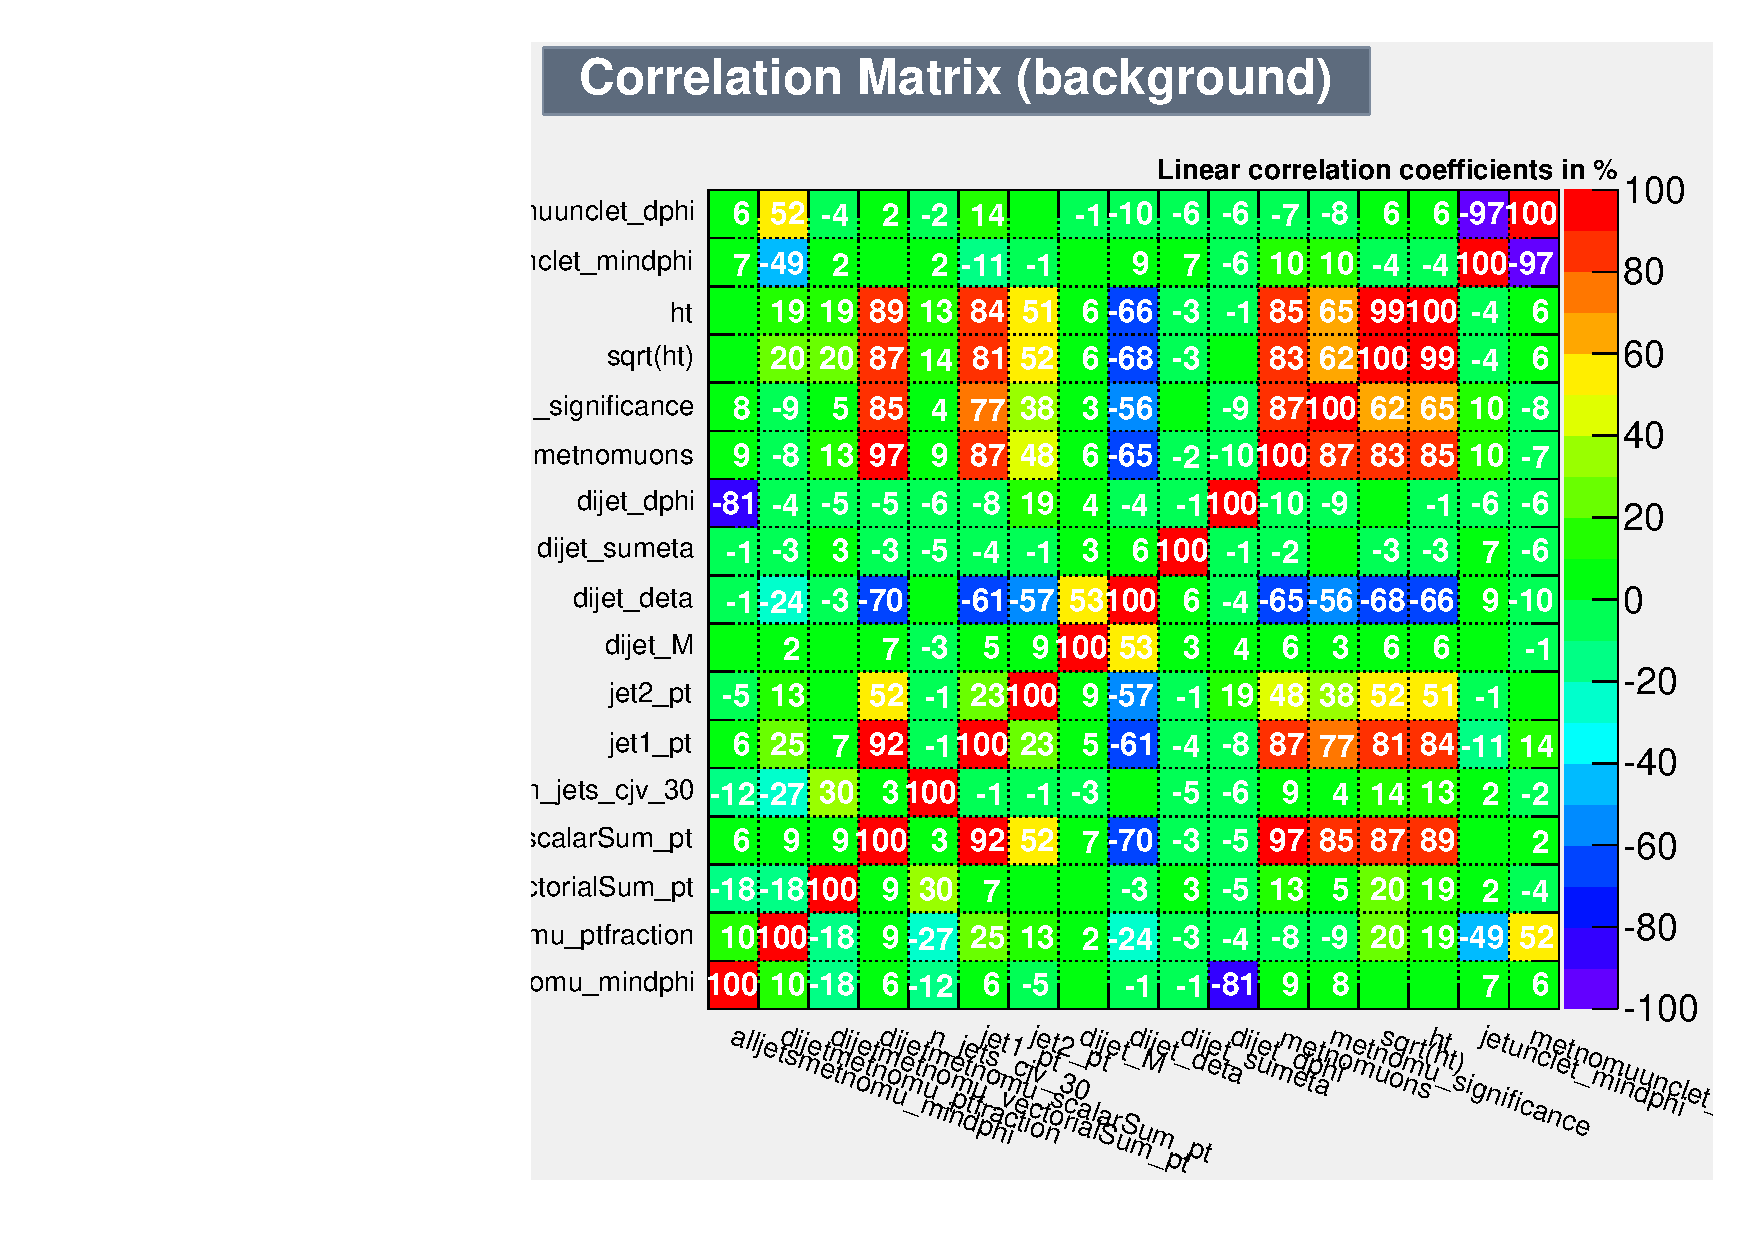
\includegraphics[width=0.5\textwidth]{TalkPics/bdt271014/bkgcorr.pdf}
\end{frame}

\begin{frame}
  \frametitle{S over root B}
  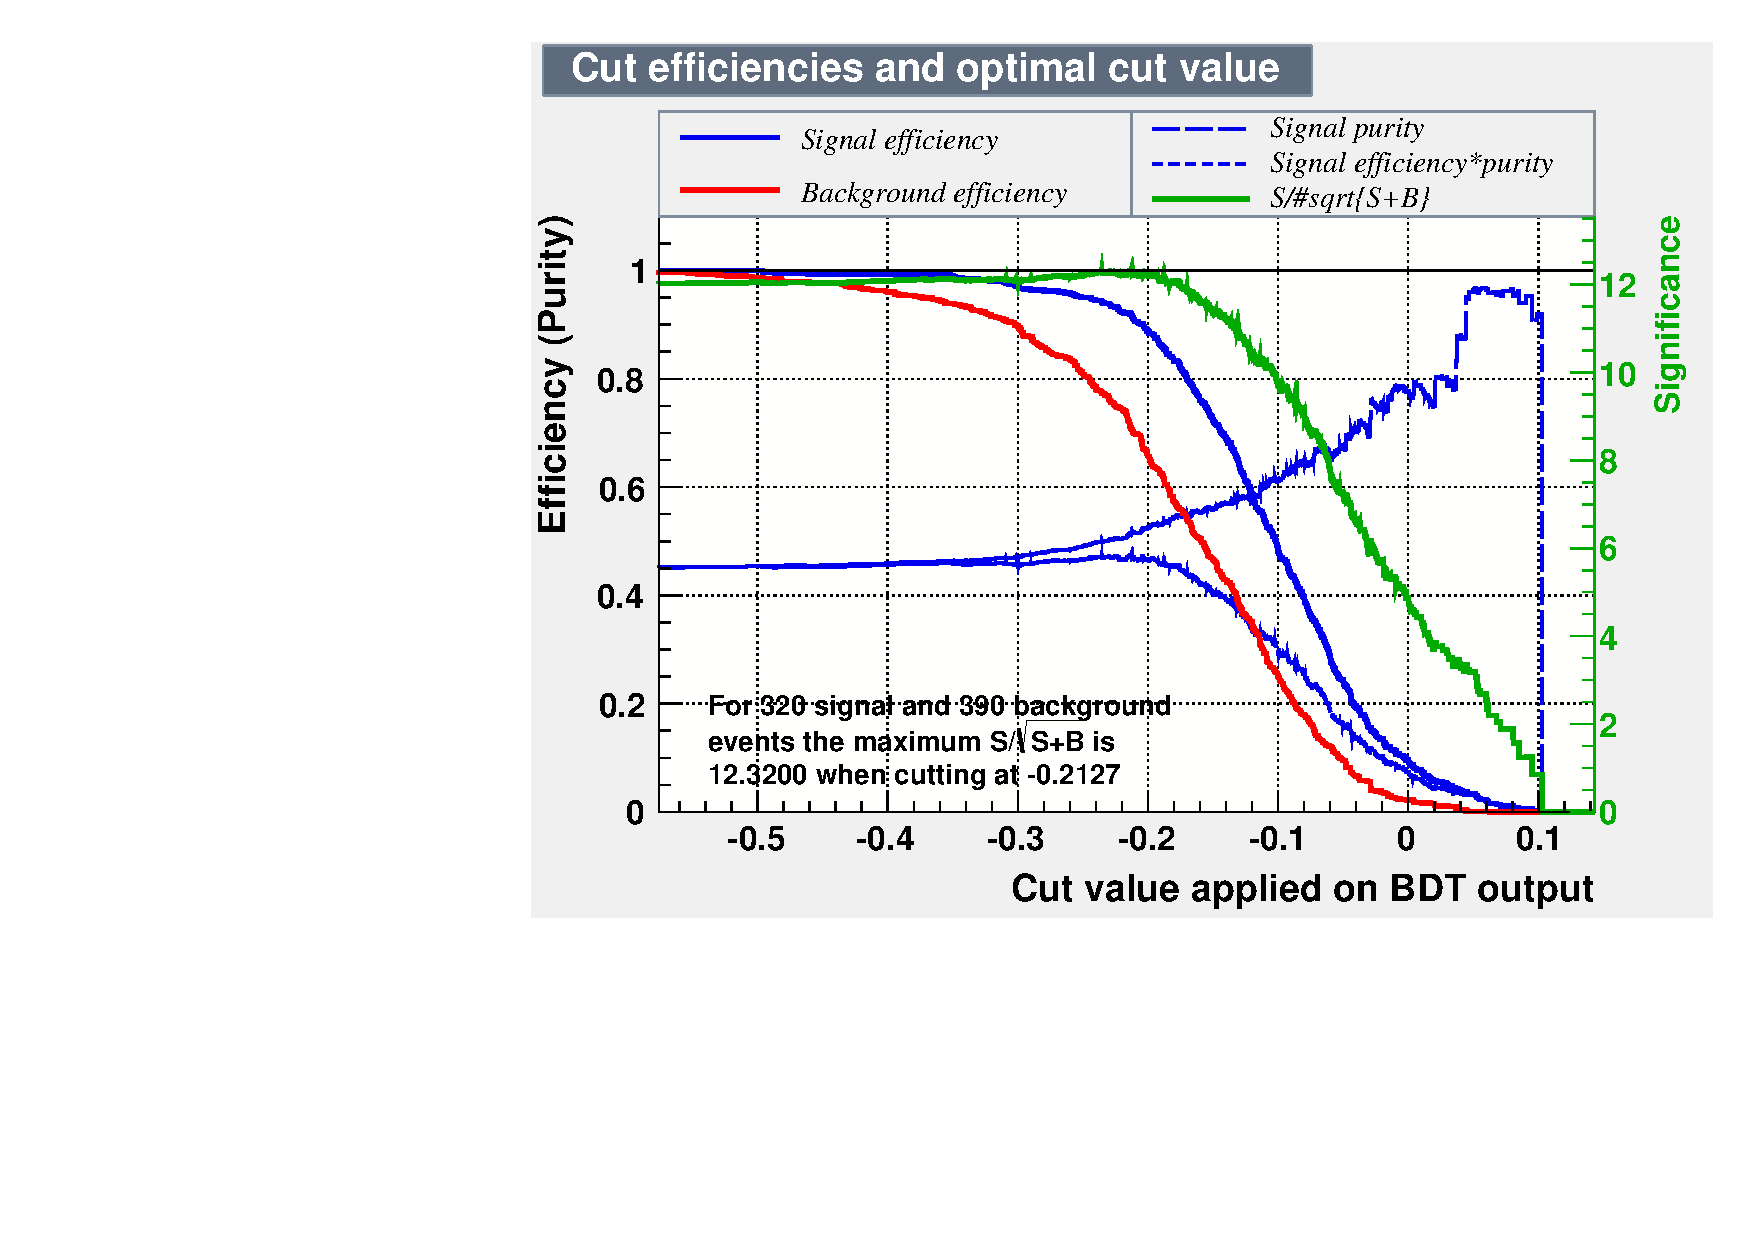
\includegraphics[width=0.5\textwidth]{TalkPics/bdt271014/bdtsoverb.pdf}
  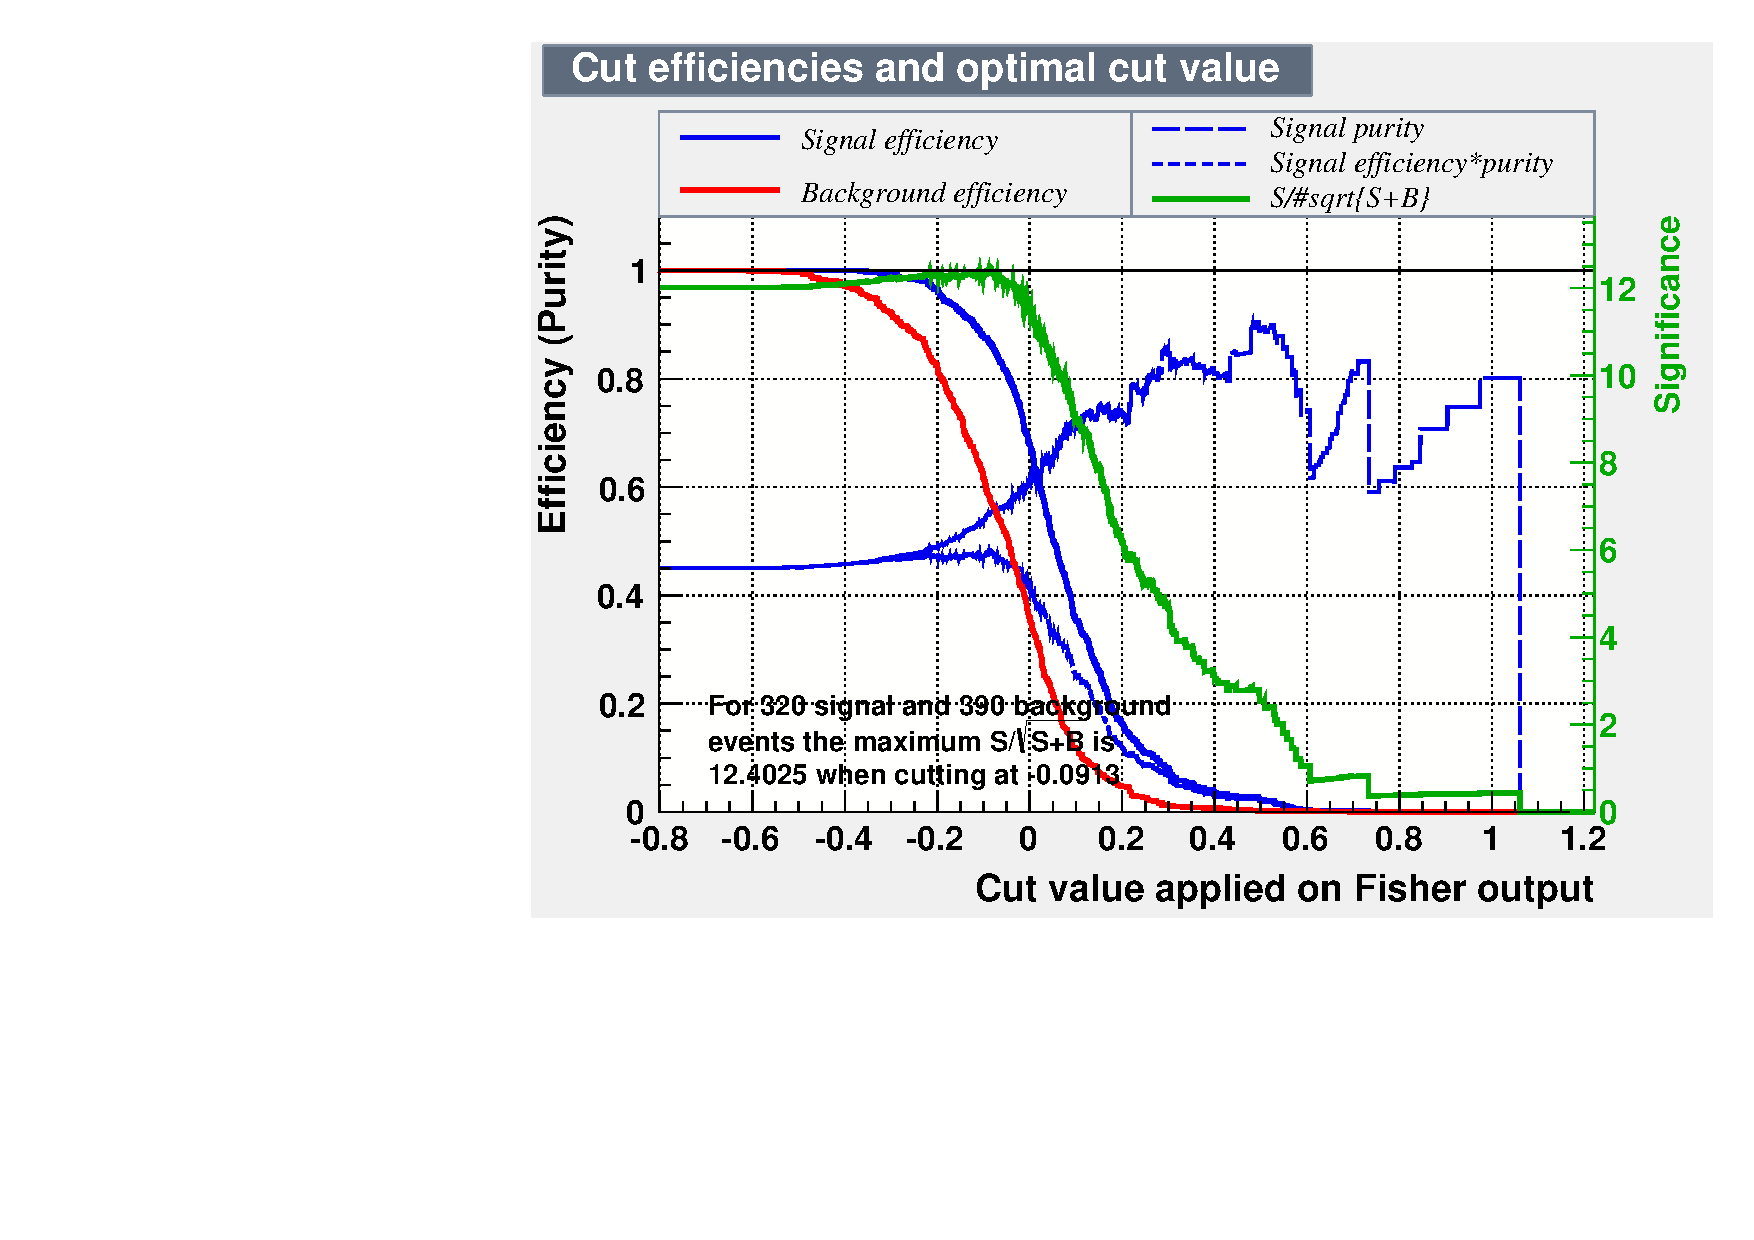
\includegraphics[width=0.5\textwidth]{TalkPics/bdt271014/fishersoverb.pdf}
\end{frame}

\begin{frame}
  \frametitle{Response}
  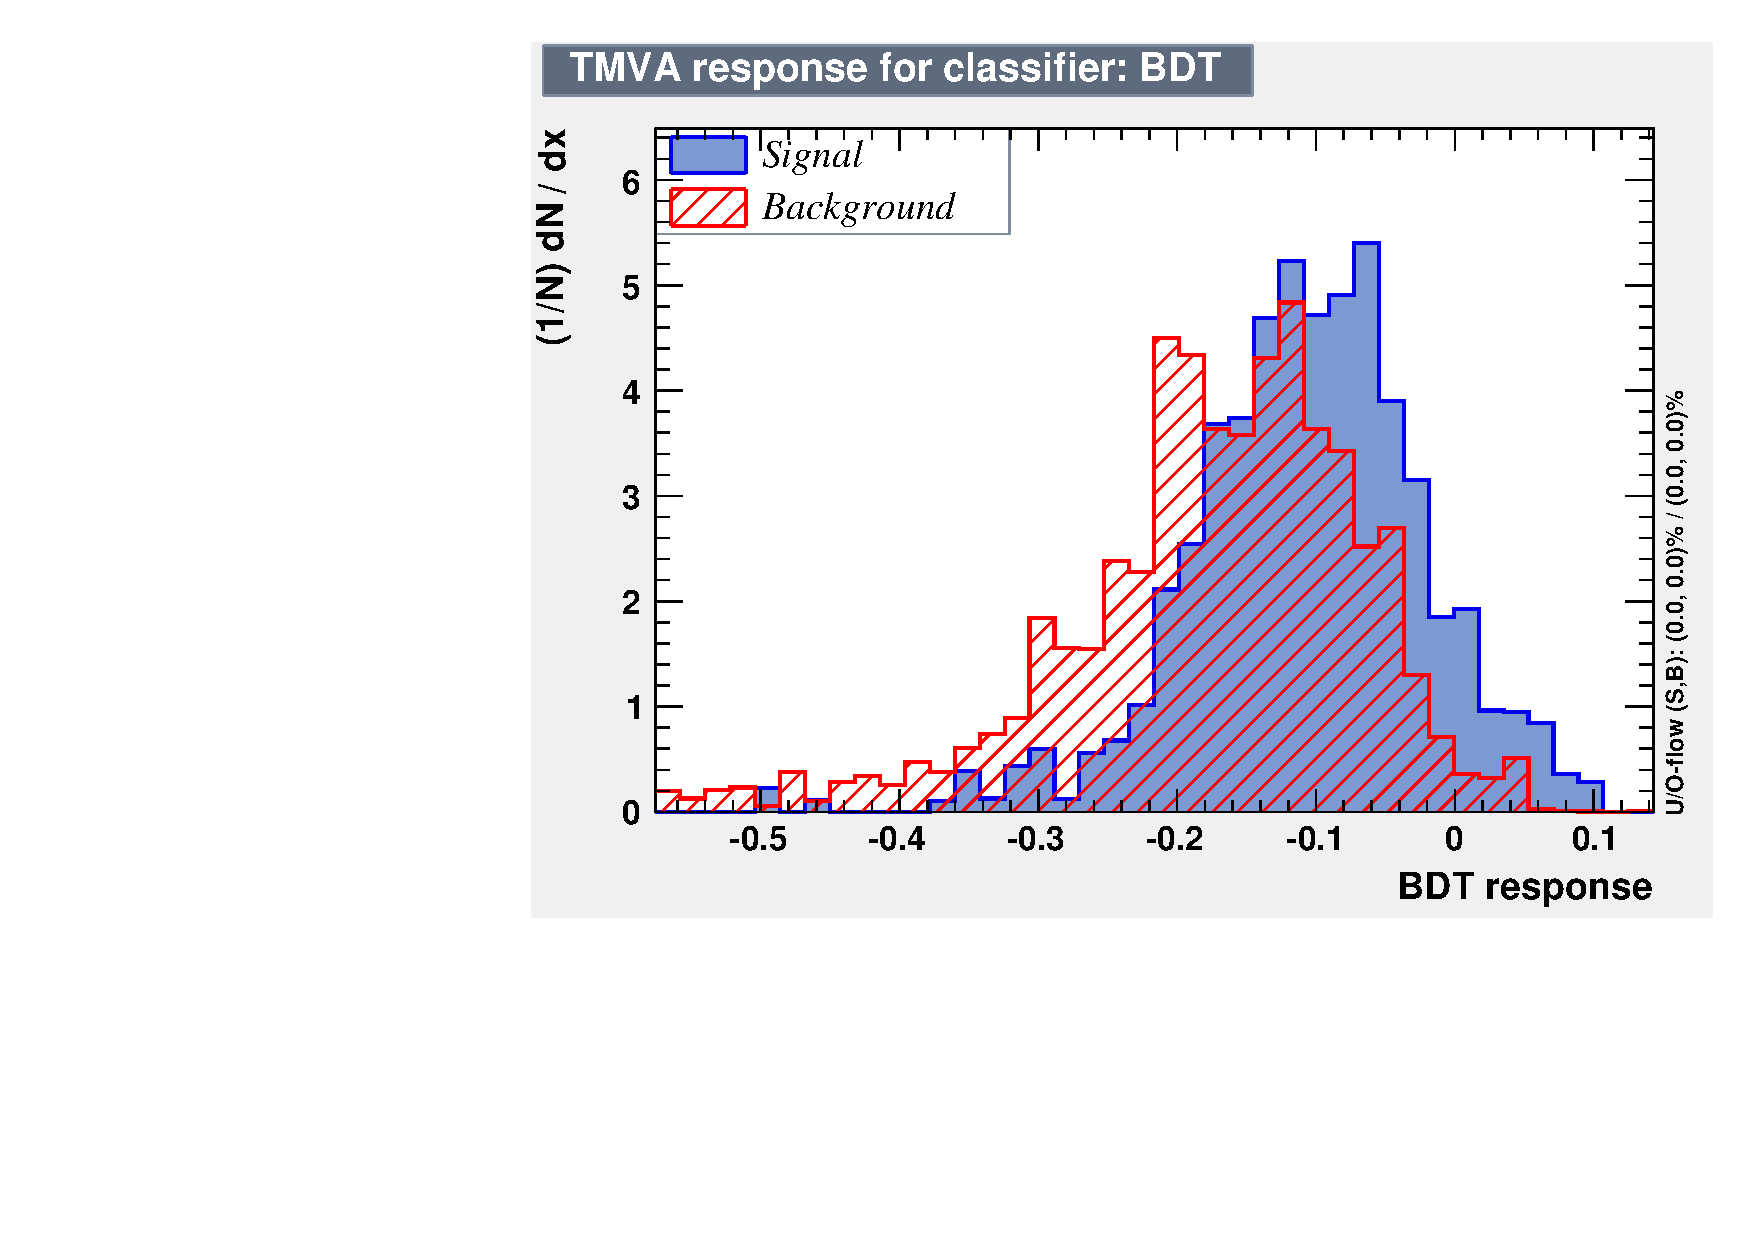
\includegraphics[width=0.5\textwidth]{TalkPics/bdt271014/bdtresponse.pdf}
  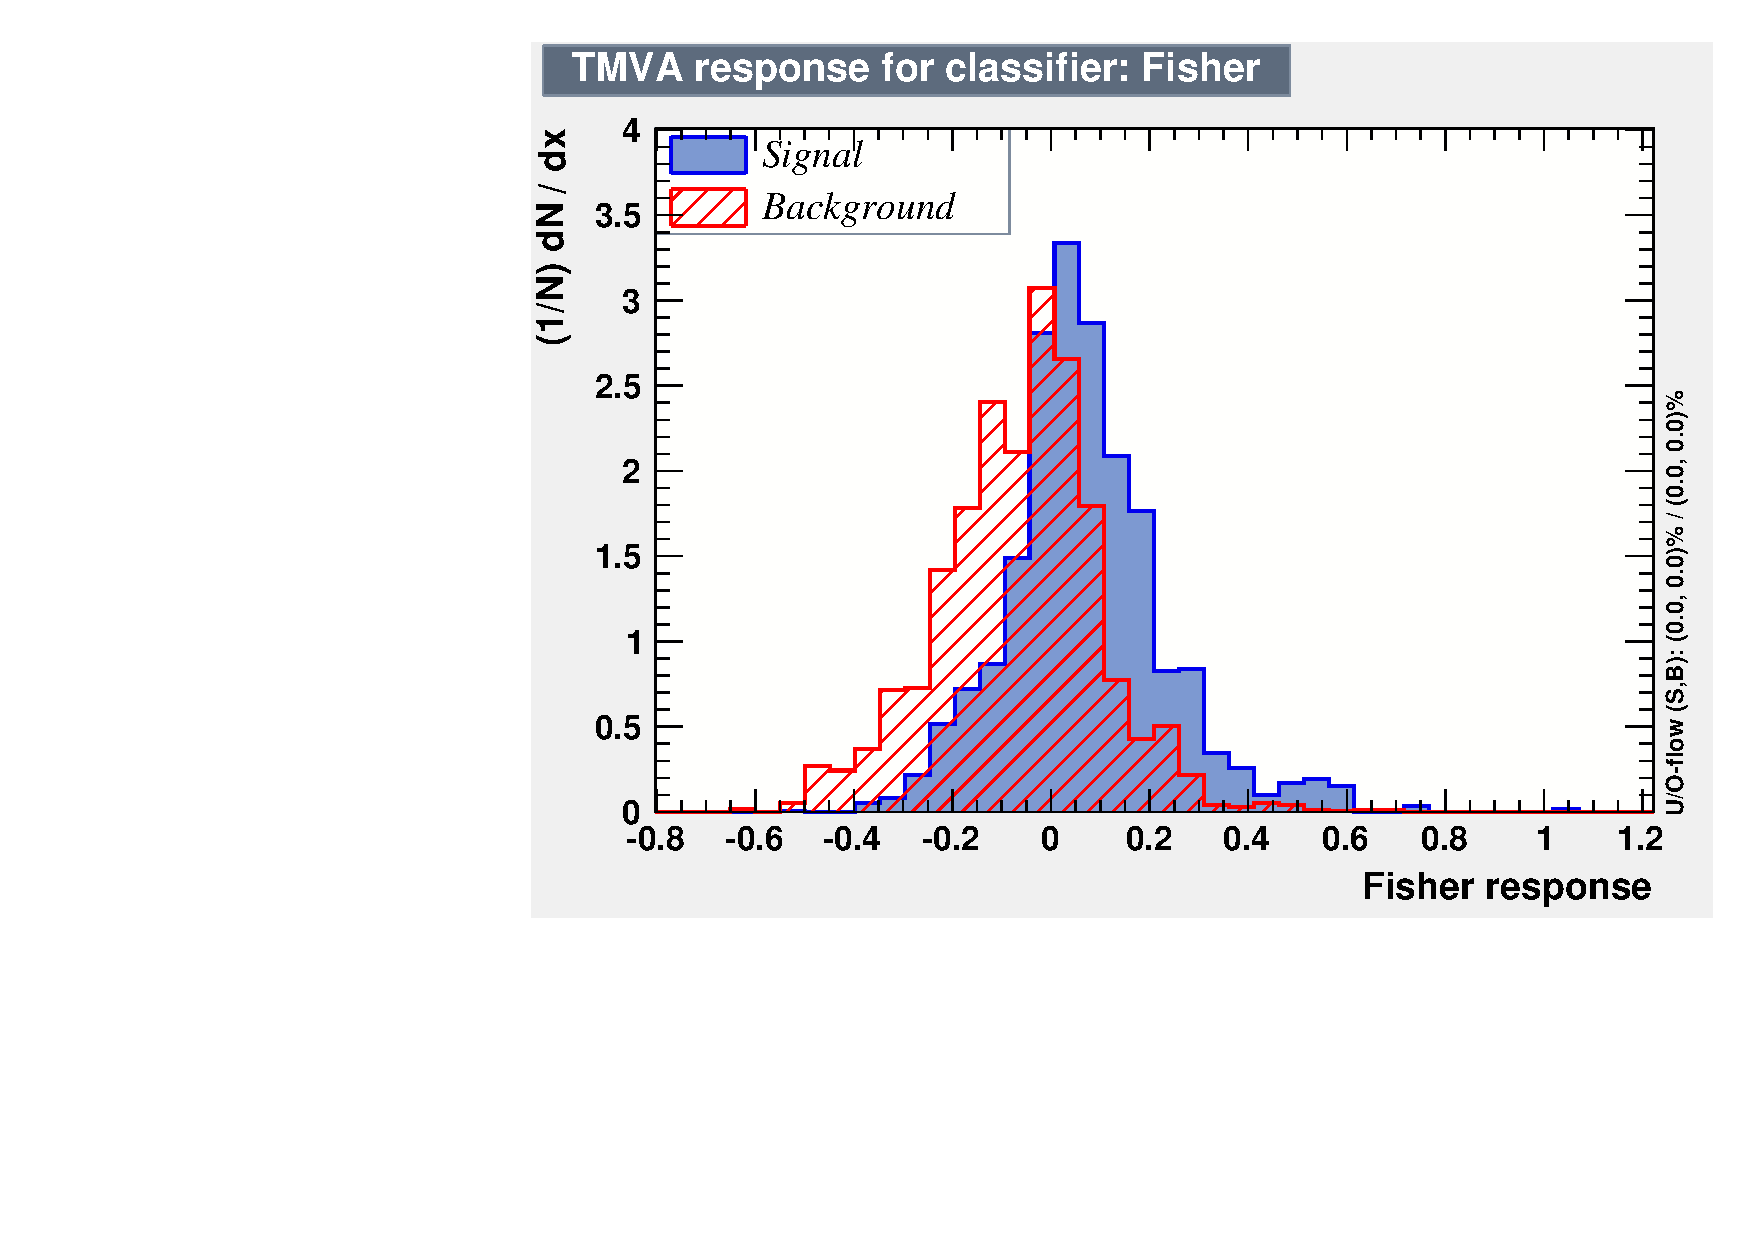
\includegraphics[width=0.5\textwidth]{TalkPics/bdt271014/fisherresponse.pdf}
\end{frame}

\begin{frame}
  \frametitle{ROC curve}
  \centering
  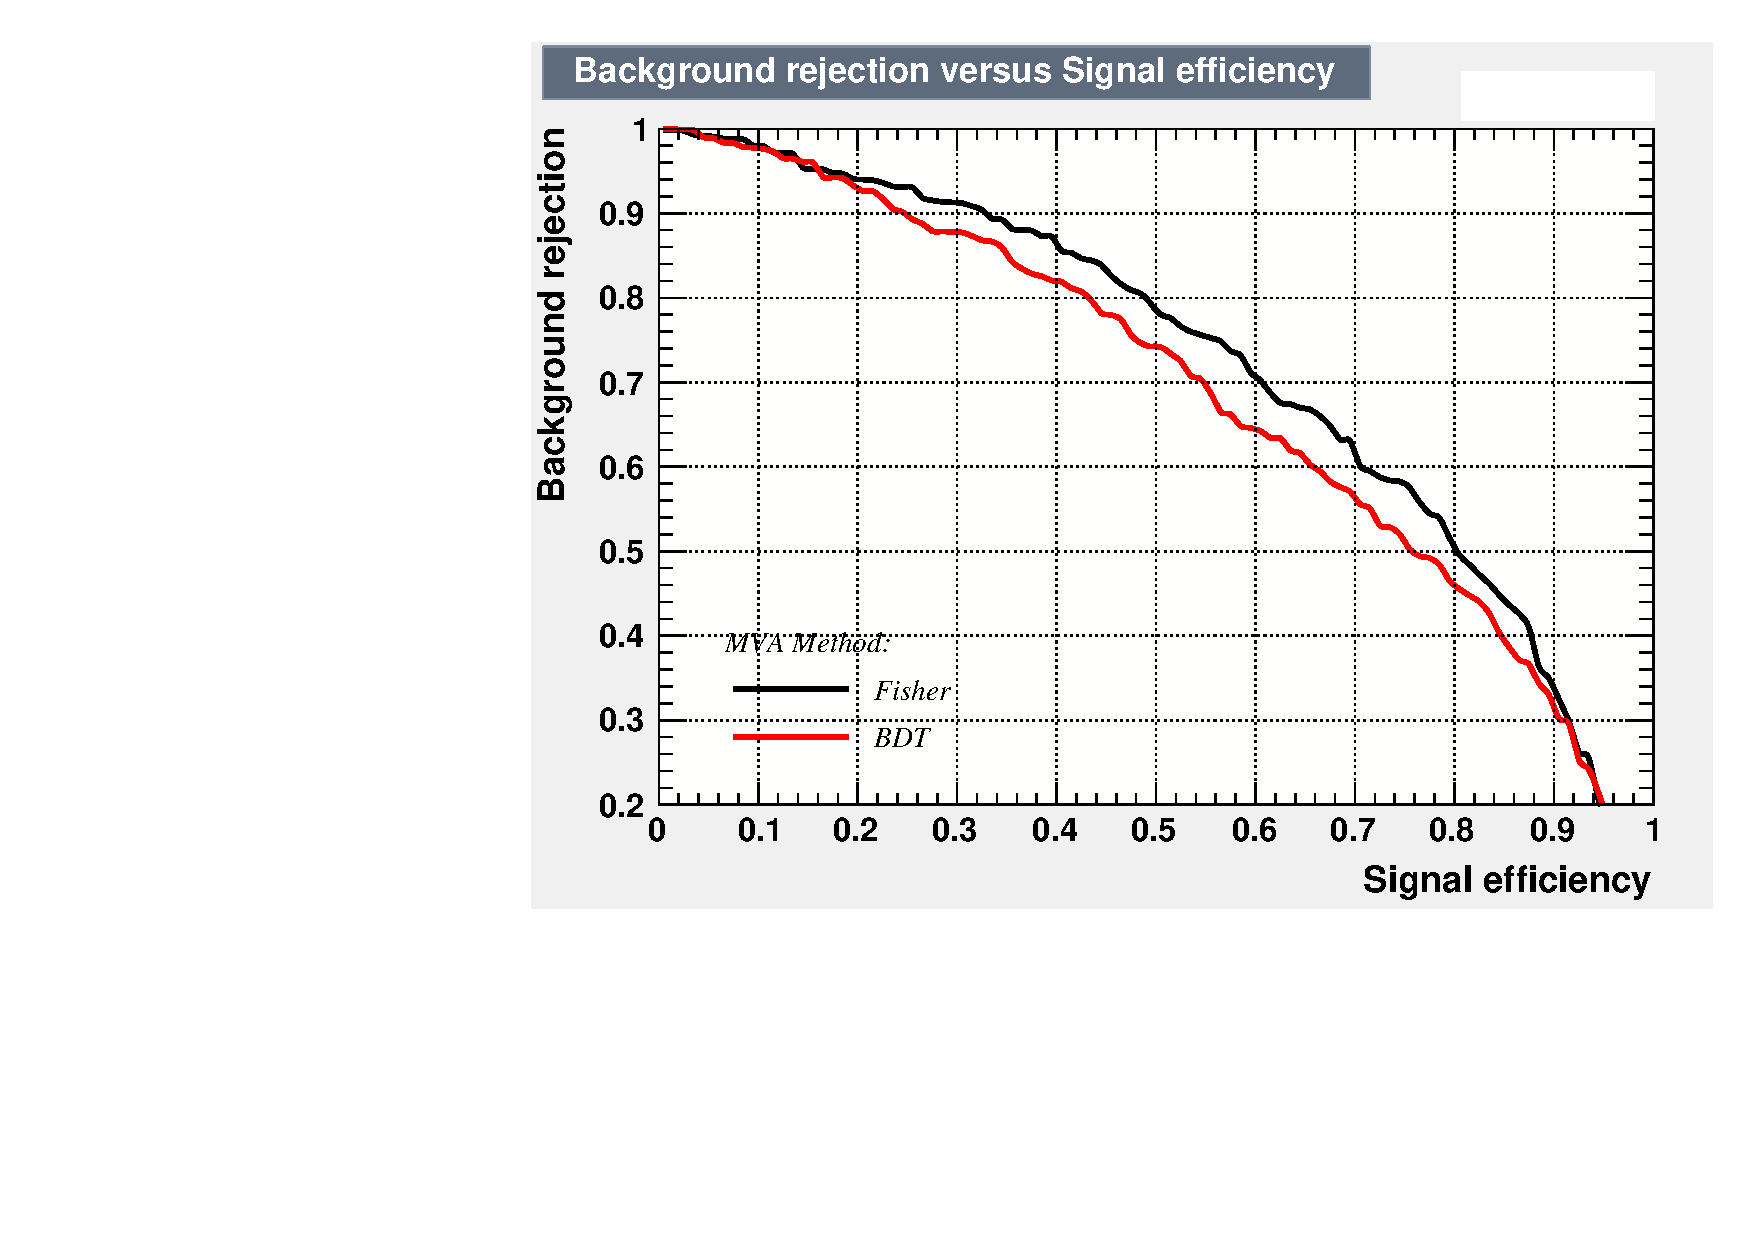
\includegraphics[width=0.8\textwidth]{TalkPics/bdt271014/roc.pdf}
\end{frame}

\begin{frame}
  \frametitle{Summary}
  \label{lastframe}

  \begin{block}{}
    \scriptsize
    \begin{itemize}
    \item Doesn't look like MVA gives much improvement in $S/\sqrt{S+B}$
    \item[-] Current cuts very tight due to ``cut all QCD'' strategy
    \item[-] All remaining backgrounds are quite signal like
    \item Need to look at expected limit
    \item This was a very quick study, any hints on things I might have missed are welcome!
    \end{itemize}
  \end{block}

\end{frame}

\begin{frame}
  \frametitle{Backup}
\end{frame}




\end{fmffile}
\end{document}
